\pgfplotsset{compat=1.9}

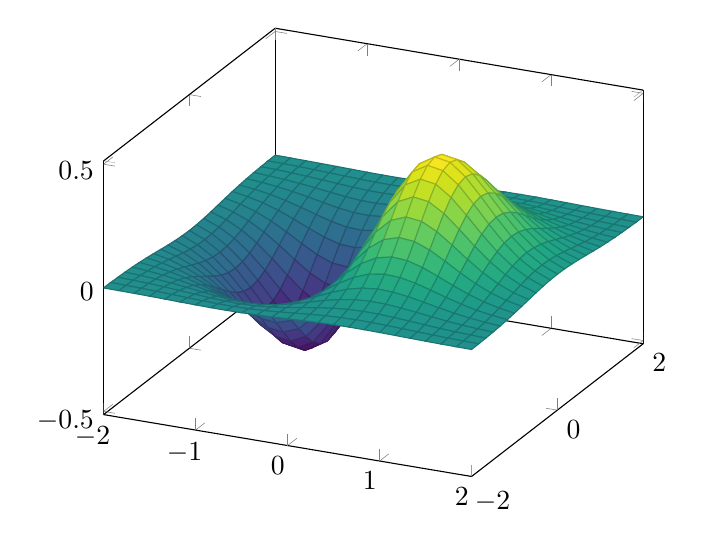
\begin{tikzpicture}
\begin{axis}%[title=Bivariate Gaussian]
   \addplot3 [surf,colormap/viridis,domain=-2:2] {x * exp(-x^2-y^2)};
\end{axis}
\end{tikzpicture}


% Try using "colormap/viridis" instead of "fill=white"
% ...done - yes - looks better - but maybe use more samples - it looks a bit rough